\section*{Problem 1}

Consider an element shown in Fig. 1 with a quadratic displacement field \( u(x) = a_1 + a_2 x + a_3 x^2 \).

\begin{figure}[h!]
    \centering
    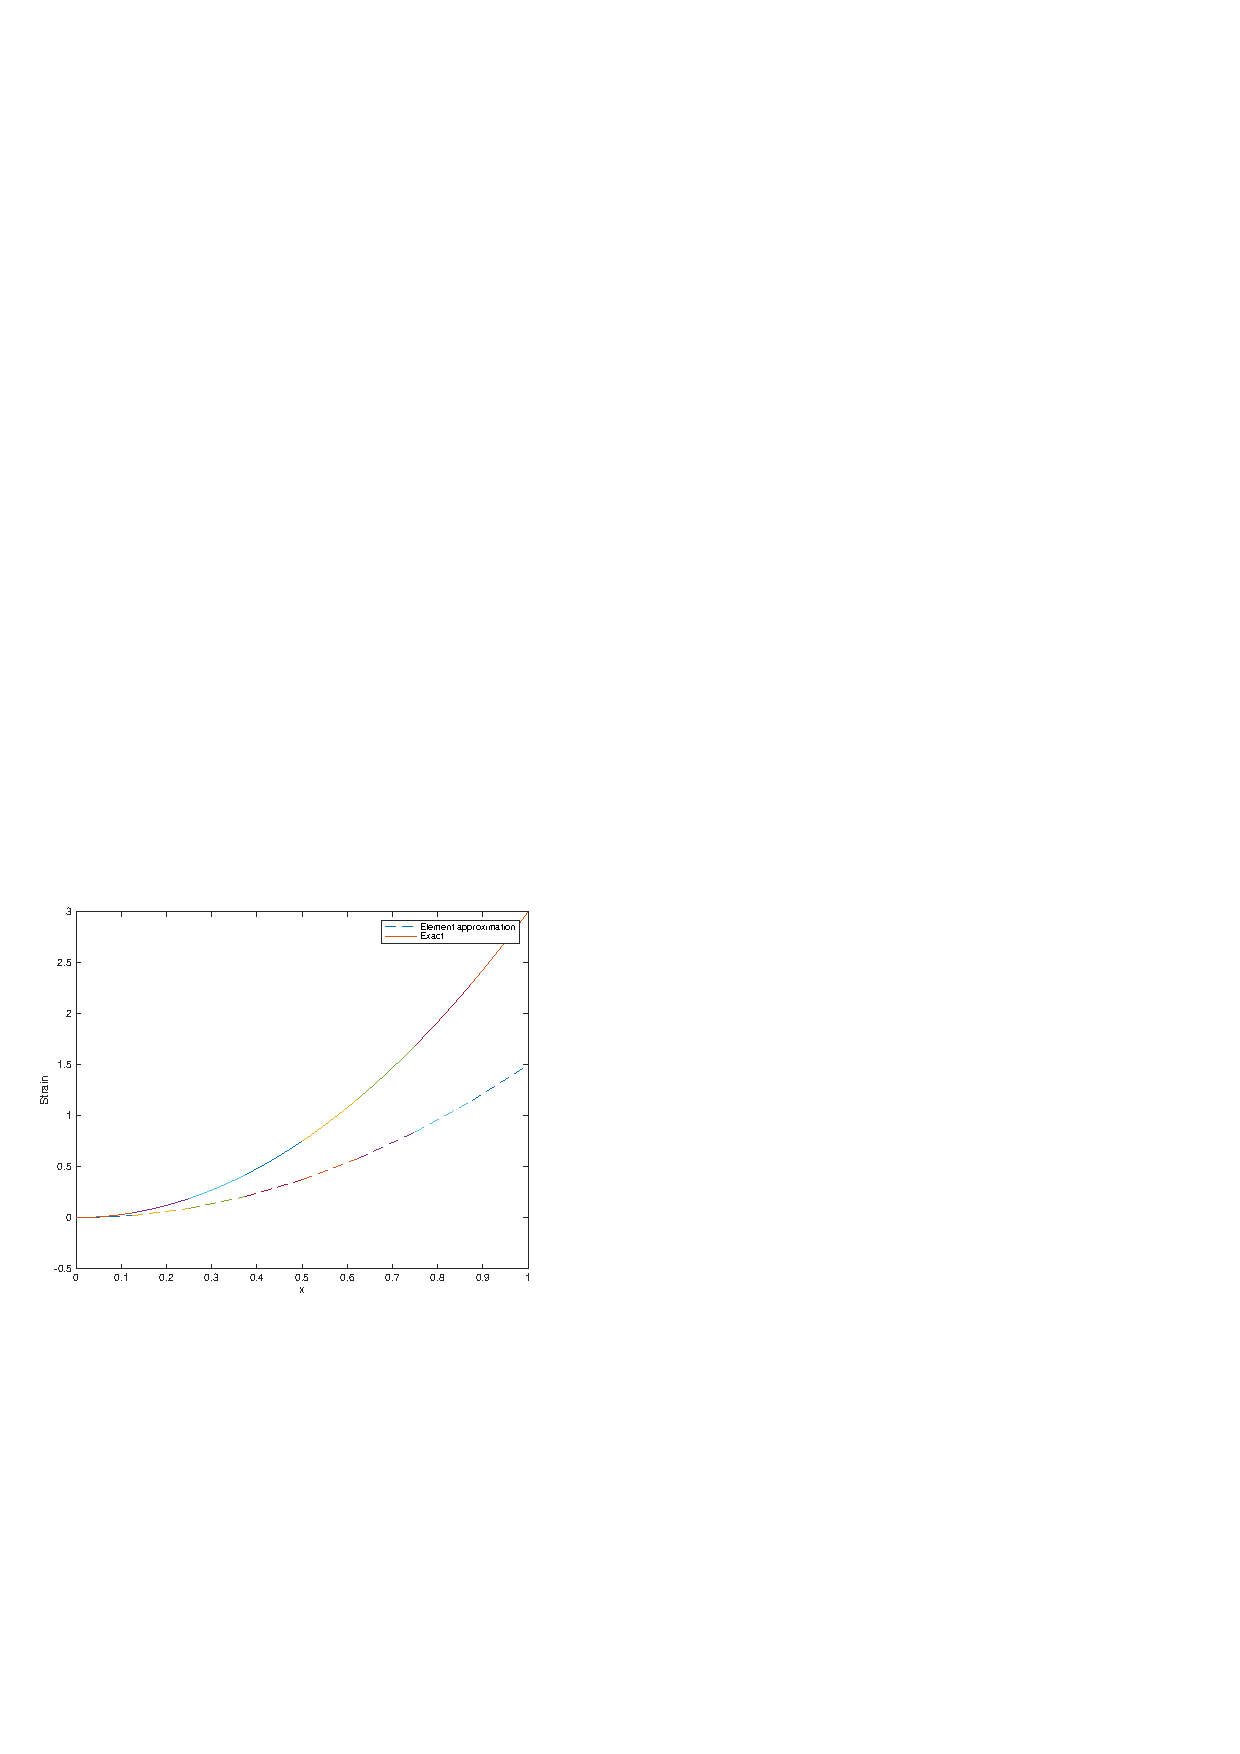
\includegraphics[width=0.5\textwidth]{figure_1.png}  % Replace with your image file name
    \caption{Problem 1}
    \label{fig:element}
\end{figure}

\begin{enumerate}
    \item[(a)] (10 points) Express the displacement field in terms of the nodal displacements \( d_1 \), \( d_2 \), and \( d_3 \). (Hint: Use the quadratic interpolants in the local coordinate \( \xi \).)
    
    \item[(b)] (5 points) For a linear body force field \( b(\xi) = b_1 \frac{1}{2}(1 - \xi) + b_3 \frac{1}{2}(1 + \xi) \), show that the external force matrix is given by 
    \[
    \mathbf{f}_e = L \begin{bmatrix} b_1 & 2(b_1 + b_3) & b_3 \end{bmatrix}^T.
    \]
    
    \item[(c)] (5 points) Develop the \( \mathbf{B}_E \) matrix such that \( \epsilon = \frac{du}{dx} = \mathbf{B}_E \mathbf{d}_E \), where \( \mathbf{d}_E = \begin{bmatrix} u_1 & u_2 & u_3 \end{bmatrix}^T \).
    
    \item[(d)] (5 points) Use one three-node quadratic element to solve, by finite elements, the differential equation \( E \frac{d^2 u}{dx^2} = -b(x) = -c x \) with boundary conditions \( u\left(-\frac{L}{2}\right) = u\left(\frac{L}{2}\right) = 0.0 \).
    
    \item[(e)] (5 points) Compare the FEM results to the exact solution for \( u(x) \) and \( \sigma(x) \).
\end{enumerate}

\subsection*{Given values for problem 1}

\begin{align}
    u_{x} &= a_{1} + a_{2}x + a_{3}x^{2} \label{eq:u_x} \\
    \xi &= \frac{2x}{L} \label{eq:xi} \\
    \xi_{1} &= -1 \label{eq:xi_1} \\
    \xi_{2} &= 0 \label{eq:xi_2} \\
    \xi_{3} &= 1 \label{eq:xi_3} \\
    N_1 &= \frac{(x - x_2)(x - x_3)}{(x_1 - x_2)(x_1 - x_3)} \label{eq:N_1} \\
    N_2 &= \frac{(x - x_1)(x - x_3)}{(x_2 - x_1)(x_2 - x_3)} \label{eq:N_2} \\
    N_3 &= \frac{(x - x_1)(x - x_2)}{(x_3 - x_1)(x_3 - x_2)} \label{eq:N_3} \\
    f_{\Omega} &= \int_{x_1}^{x_2} N^{eT} b \, dx \label{eq:f_Omega} \\
    J &= \frac{dx}{d\xi} \label{eq:jacobian}
\end{align}

\subsection*{a.$)$ Express the displacement field in terms of the nodal displacements \( d_1, d_2, d_3 \).}

\subsubsection*{Lagrange Interpolations of the Shape Functions}

Let's find the shape functions with respect to \( \xi \) by substituting equations \eqref{eq:xi_1}, \eqref{eq:xi_2}, and \eqref{eq:xi_3} into equations \eqref{eq:N_1}, \eqref{eq:N_2}, and \eqref{eq:N_3}.

\begin{align}
    N_1(\xi) &= \frac{\xi (1 - \xi)}{2} \\
    N_2(\xi) &= 1 - \xi^2 \\
    N_3(\xi) &= \frac{\xi (1 + \xi)}{2}
\end{align}

These values can be confirmed by the interpolation property and the partition of unity:
\begin{equation*}
    N_i(\xi_j) = \delta_{ij}
\end{equation*}

\begin{equation*}
    \sum_{i=1}^{3} N_i(\xi) = 1
\end{equation*}

\subsubsection*{Interpolated Function}

If \( d_1 \), \( d_2 \), and \( d_3 \) are the values of the distribution \( u \) at the nodes, the quadratic interpolation \( u(\xi) \) over the element in local coordinates can be expressed as:

\begin{equation}
    u(\xi) = N_1(\xi) d_1 + N_2(\xi) d_2 + N_3(\xi) d_3
    \label{eq:displacement}
\end{equation}

Substituting the equations \( N_1 \), \( N_2 \), and \( N_3 \) into the function, we get:

\begin{equation}
    u(\xi) = \frac{1}{2} \xi (\xi - 1) d_1 + (1 - \xi^2) d_2 + \frac{1}{2} \xi (\xi + 1) d_3
\end{equation}

Substituting \( \xi = \frac{2x}{L} \) into this expression:

\begin{equation}
    u(x) = \frac{1}{L^2}\left[ x(2x - L) d_1 + \left( L^2 - 4x^2 \right) d_2 + x(2x + L) d_3 \right]
\end{equation}

\subsection*{b.$)$ Show that the external force matrix is given by \( \mathbf{f}_e = \frac{L}{6} \begin{bmatrix} b_1 \\ 2(b_1 + b_3) \\ b_3 \end{bmatrix} \).}

To show this, we calculate the external force matrix \( \mathbf{f}_e \) using the body force \( b(\xi) = b_1 \frac{1}{2}(1 - \xi) + b_3 \frac{1}{2}(1 + \xi) \) and adjusting with the Jacobian term.

\subsection*{c.$)$}

Develop the \( \mathbf{B}_E \) matrix such that:

\begin{equation}
    \epsilon = \frac{du}{dx} = \mathbf{B}_E \, \mathbf{d}_E
\end{equation}

where

\begin{equation}
    \mathbf{d}_E = \begin{bmatrix} u_1 \\ u_2 \\ u_3 \end{bmatrix}^T
\end{equation}

The displacement field can be represented in local notation from \eqref{eq:displacement}.
We are told that \( \epsilon = \frac{du}{dx} \); however, our function is in terms of \( \xi \).
So, to get \( \frac{du}{dx} \) from a function dependent on \( \xi \), we use the chain rule:

\begin{equation}
    \epsilon = \frac{du}{dx} = \frac{dN_1}{d\xi} \frac{d\xi}{dx} u_1 + \frac{dN_2}{d\xi} \frac{d\xi}{dx} u_2 + \frac{dN_3}{d\xi} \frac{d\xi}{dx} u_3
\end{equation}

The Jacobian \eqref{eq:jacobian} shows that \( \frac{d\xi}{dx} = \frac{L}{2} \), so we only need to find \( \frac{dN}{d\xi} \).

\subsection*{Derivatives of Shape Functions with Respect to \( x \)}

Using the chain rule, each derivative \( \frac{dN_i}{dx} \) can be expressed as:

\[
\frac{dN_i}{dx} = \frac{dN_i}{d\xi} \cdot \frac{2}{L}
\]

For each shape function:

1. **For \( N_1(\xi) \):**
   \[
   \frac{dN_1}{d\xi} = \xi - \frac{1}{2} \Rightarrow \frac{dN_1}{dx} = \frac{2}{L} \left( \xi - \frac{1}{2} \right)
   \]

2. **For \( N_2(\xi) \):**
   \[
   \frac{dN_2}{d\xi} = -2\xi \Rightarrow \frac{dN_2}{dx} = -\frac{4\xi}{L}
   \]

3. **For \( N_3(\xi) \):**
   \[
   \frac{dN_3}{d\xi} = \xi + \frac{1}{2} \Rightarrow \frac{dN_3}{dx} = \frac{2}{L} \left( \xi + \frac{1}{2} \right)
   \]

\subsection*{Constructing the \( \mathbf{B}_E \) Matrix}

Using the derivatives calculated above, we can now construct the \( \mathbf{B}_E \) matrix:

\begin{equation}
    \mathbf{B}_E = \begin{bmatrix} \frac{2}{L} \left( \xi - \frac{1}{2} \right) & -\frac{4\xi}{L} & \frac{2}{L} \left( \xi + \frac{1}{2} \right) \end{bmatrix}
\end{equation}

This matrix \( \mathbf{B}_E \) now relates the nodal displacement vector \( \mathbf{d}_E \) to the strain \( \epsilon \) within the element:

\begin{equation}
    \epsilon = \mathbf{B}_E \, \mathbf{d}_E
\end{equation}

\subsection*{d.$)$ Calculate the element stiffness matrix.}

The element stiffness matrix \( \mathbf{K}^e \) for a one-dimensional bar element in the finite element method is expressed as:

\begin{equation}
    \mathbf{K}^e = \int_{-1}^{1} (\mathbf{B}^e)^T E A \, \mathbf{B}^e \, J \, d\xi
\end{equation}

where \( J = \frac{L}{2} \) is the Jacobian.

\subsubsection*{Final Stiffness Matrix}

After integration, the stiffness matrix is:

\begin{equation}
    \mathbf{K}^e = \frac{A E}{3 L} \begin{bmatrix} 7 & -8 & 1 \\ -8 & 16 & -8 \\ 1 & -8 & 7 \end{bmatrix}
\end{equation}

\subsection*{e.$)$ Comparison of FEM Results to the Exact Solution}

To validate, compare FEM values for \( u(x) \) and \( \sigma(x) \) with exact solutions for accuracy.

\subsection*{Verification of Shape Functions \( N_1, N_2, \) and \( N_3 \)}

\subsubsection*{Verification for \( N_1(\xi) \)}

\begin{align*}
    N_1(-1) &= \frac{1}{2}(-1)(-1 - 1) \\
            &= \frac{1}{2}(-1)(-2) \\
            &= \frac{1}{2} \cdot 2 \\
            &= \frac{2}{2} \\
            &= 1
\end{align*}

\begin{align*}
    N_1(0) &= \frac{1}{2}(0)(0 - 1) \\
           &= \frac{1}{2} \cdot 0 \\
           &= 0
\end{align*}

\begin{align*}
    N_1(1) &= \frac{1}{2}(1)(1 - 1) \\
           &= \frac{1}{2} \cdot 0 \\
           &= 0
\end{align*}

\subsubsection*{Verification for \( N_2(\xi) \)}

\begin{align*}
    N_2(-1) &= 1 - (-1)^2 \\
            &= 1 - 1 \\
            &= 0
\end{align*}

\begin{align*}
    N_2(0) &= 1 - (0)^2 \\
           &= 1 - 0 \\
           &= 1
\end{align*}

\begin{align*}
    N_2(1) &= 1 - (1)^2 \\
           &= 1 - 1 \\
           &= 0
\end{align*}

\subsubsection*{Verification for \( N_3(\xi) \)}

\begin{align*}
    N_3(-1) &= \frac{1}{2}(-1)(-1 + 1) \\
            &= \frac{1}{2}(-1)(0) \\
            &= 0
\end{align*}

\begin{align*}
    N_3(0) &= \frac{1}{2}(0)(0 + 1) \\
           &= \frac{1}{2} \cdot 0 \\
           &= 0
\end{align*}

\begin{align*}
    N_3(1) &= \frac{1}{2}(1)(1 + 1) \\
           &= \frac{1}{2}(1)(2) \\
           &= \frac{2}{2} \\
           &= 1
\end{align*}

This confirms the shape functions for each node.

\subsubsection*{Interpolated Function for \( u(x) \)}

If \( d_1 \), \( d_2 \), and \( d_3 \) are the values of the distribution \( u \) at the nodes, the quadratic interpolation \( u(\xi) \) over the element in local coordinates can be expressed as:

\begin{equation}
    u(\xi) = N_1(\xi) d_1 + N_2(\xi) d_2 + N_3(\xi) d_3
\end{equation}

Substituting the equations \( N_1 \), \( N_2 \), and \( N_3 \) into the function we get:

\begin{equation}
    u(\xi) = \frac{1}{2} \xi (\xi - 1) d_1 + (1 - \xi^2) d_2 + \frac{1}{2} \xi (\xi + 1) d_3
\end{equation}

\subsubsection*{Transforming \( u(\xi) \) to \( u(x) \)}

The problem gives us the value for \( \xi = \frac{2x}{L} \). So to finalize the displacement field we substitute and simplify:

\begin{align*}
    u(x) &= \frac{1}{2} \left( \frac{2x}{L} \right) \left( \frac{2x}{L} - 1 \right) d_1 + \left( 1 - \left( \frac{2x}{L} \right)^2 \right) d_2 + \frac{1}{2} \left( \frac{2x}{L} \right) \left( \frac{2x}{L} + 1 \right) d_3 \\
    &= \frac{2x (2x - L)}{2L^2} \, d_1 + \left( \frac{L^2 - 4x^2}{L^2} \right) d_2 + \frac{2x (2x + L)}{2L^2} \, d_3 \\
    &= \frac{2x^2 - xL}{L^2} \, d_1 + \frac{L^2 - 4x^2}{L^2} \, d_2 + \frac{2x^2 + xL}{L^2} \, d_3
\end{align*}

Thus, the simplified form of \( u(x) \) is:

\begin{equation*}
    u(x) = \frac{1}{L^2}\left[ x(2x-L)  \, d_1 + \left( L^{2}-4x^2 \right) \, d_2 + \left( x(2x+L) \right) \, d_3 \right]
\end{equation*}

\subsection*{External Force Matrix Calculation}

For a linear body force field \( b(\xi) = b_1 \frac{1}{2}(1 - \xi) + b_3 \frac{1}{2}(1 + \xi) \), we proceed to show that the external force matrix is given by:

\[
\mathbf{f}_e = \frac{L}{6} \begin{bmatrix} b_1 \\ 2(b_1 + b_3) \\ b_3 \end{bmatrix}.
\]

Using the previously defined shape functions and applying the force distribution across nodes.

\subsubsection*{The Jacobian}

The Jacobian for transforming the integral is calculated as follows:

\begin{equation*}
    J = \frac{\Delta x}{\Delta \xi} = \frac{L}{2}
\end{equation*}

Using this Jacobian, the integral calculations can be adjusted accordingly for the external force components.

\subsection*{The \( \mathbf{B}_e \) Matrix Calculation for Strain}

Given \( \epsilon = \frac{du}{dx} = \mathbf{B}_E \mathbf{d}_E \), we calculate \( \mathbf{B}_e \) using derivatives of shape functions with respect to \( \xi \).

\subsubsection*{Derivatives of Shape Functions with Respect to \( x \)}

Using the chain rule, each derivative \( \frac{dN_i}{dx} \) can be expressed as:

\[
\frac{dN_i}{dx} = \frac{dN_i}{d\xi} \cdot \frac{2}{L}
\]

For each shape function, the corresponding derivatives yield the matrix \( \mathbf{B}_e \):

\begin{equation}
    \mathbf{B}_e = \begin{bmatrix} \frac{2}{L} \left( \xi - \frac{1}{2} \right) & -\frac{4\xi}{L} & \frac{2}{L} \left( \xi + \frac{1}{2} \right) \end{bmatrix}
\end{equation}

\subsection*{d.$)$ Element Stiffness Matrix Calculation}

The element stiffness matrix \( \mathbf{K}^e \) for a one-dimensional bar element in the finite element method is expressed as:

\begin{equation}
    \mathbf{K}^e = \int_{-1}^{1} (\mathbf{B}^e)^T E A \, \mathbf{B}^e \, J \, d\xi
\end{equation}

where \( J = \frac{L}{2} \) is the Jacobian, which converts the integral in the natural coordinate \( \xi \) to the physical length.

\subsubsection*{Substituting \( \mathbf{B}^e \) and the Jacobian}

The \( \mathbf{B}^e \) matrix, as derived previously, is:

\begin{equation}
    \mathbf{B}^e = \begin{bmatrix} \frac{2}{L} \left( \xi - \frac{1}{2} \right) & -\frac{4\xi}{L} & \frac{2}{L} \left( \xi + \frac{1}{2} \right) \end{bmatrix}
\end{equation}

Now, \( \mathbf{K}^e \) can be expressed as:

\begin{equation}
    \mathbf{K}^e = \int_{-1}^{1} (\mathbf{B}^e)^T E A \mathbf{B}^e \cdot \frac{L}{2} \, d\xi
\end{equation}

The \( \frac{L}{2} \) factor comes from the Jacobian \( J \).

\subsubsection*{1. Expanding and Integrating the Stiffness Matrix}

The expanded form of \( \mathbf{K}^e \) with integration over \( \xi \) yields the matrix:

\begin{equation}
    \mathbf{K}^e = \frac{A E}{3 L} \begin{bmatrix} 7 & -8 & 1 \\ -8 & 16 & -8 \\ 1 & -8 & 7 \end{bmatrix}
\end{equation}

\subsection*{e.$)$ Comparison of FEM Results to the Exact Solution for \( u(x) \) and \( \sigma(x) \)}

To validate the accuracy of the finite element method (FEM) solution, we compare the FEM results for \( u(x) \) (displacement) and \( \sigma(x) \) (stress) with the exact analytical solution.

\begin{itemize}
    \item \textbf{Displacement, \( u(x) \):} Compare the FEM-derived displacement values at the nodes and within the element with the exact solution for \( u(x) \).
    \item \textbf{Stress, \( \sigma(x) \):} Similarly, evaluate the FEM stress distribution \( \sigma(x) = E \frac{du}{dx} \) against the exact stress profile derived from the analytical solution.
\end{itemize}

This comparison provides insight into the accuracy of the FEM approximation for both displacement and stress in the given element.

\subsection*{f.$)$ Comparison of FEM Results to Exact Solution for Stress \( \sigma(x) \)}

To ensure consistency, further validation involves comparing \( \sigma(x) \) values obtained by FEM and exact solutions for precision.

\subsubsection*{Exact Solution for \( u(x) \)}

Given the differential equation:
\[
E \frac{d^2 u}{dx^2} = -c x,
\]
with boundary conditions \( u\left(-\frac{L}{2}\right) = 0 \) and \( u\left(\frac{L}{2}\right) = 0 \), we can integrate to obtain the exact solution.

\paragraph{First Integration:} Integrate once with respect to \( x \) to find the slope (or strain) \( \frac{du}{dx} \):
\[
E \frac{du}{dx} = -\frac{c x^2}{2} + C_1,
\]
where \( C_1 \) is a constant of integration.

\paragraph{Second Integration:} Integrate again to find \( u(x) \):
\[
E u(x) = -\frac{c x^3}{6} + C_1 x + C_2,
\]
where \( C_2 \) is another constant of integration.

\paragraph{Applying Boundary Conditions:} Using \( u\left(-\frac{L}{2}\right) = 0 \) and \( u\left(\frac{L}{2}\right) = 0 \), we solve for \( C_1 \) and \( C_2 \):

At \( x = -\frac{L}{2} \):
\[
0 = -\frac{c}{6}\left(-\frac{L}{2}\right)^3 + C_1\left(-\frac{L}{2}\right) + C_2.
\]

At \( x = \frac{L}{2} \):
\[
0 = -\frac{c}{6}\left(\frac{L}{2}\right)^3 + C_1\left(\frac{L}{2}\right) + C_2.
\]

Solving these, we find \( C_1 = 0 \) and \( C_2 = \frac{c L^3}{48 E} \).

\paragraph{Exact Solution for \( u(x) \):}
\[
u(x) = \frac{c}{6 E} \left(\frac{L^2}{4} x - \frac{x^3}{3}\right).
\]

\subsubsection*{Exact Solution for \( \sigma(x) \)}

Stress \( \sigma(x) \) is related to the strain \( \frac{du}{dx} \) by:
\[
\sigma(x) = E \frac{du}{dx}.
\]
From our first integration, we have:
\[
\sigma(x) = -\frac{c x^2}{2}.
\]

\subsubsection*{Displacement Comparison}

\begin{enumerate}
    \item \textbf{FEM Displacements:} 
        \begin{align*}
            u_{FEM}(-L/2) &= 0 \quad \text{and} \quad u_{FEM}(L/2) = 0 \quad \text{(boundary conditions)}, \\
            u_{FEM}(0) &= u_2 \quad \text{from the FEM solution}.
        \end{align*}

    \item \textbf{Exact Displacement:}
        \begin{align*}
            u_{exact}(x) &= \frac{c}{6E} \left(\frac{L^2}{4} x - \frac{x^3}{3}\right), \\
            u_{exact}(0) &= \frac{c L^2}{24E} \quad \text{(at } x = 0\text{)}, \\
            u_{exact} &= 0 \quad \text{(at } x = -L/2 \text{ and } x = L/2\text{)}.
        \end{align*}

    \item \textbf{Comparison:} The FEM solution matches the exact solution at the boundary points. At \( x = 0 \), compare \( u_{FEM}(0) = u_2 \) with \( u_{exact}(0) = \frac{c L^2}{24E} \).
\end{enumerate}

\subsubsection*{Stress Comparison}

\begin{enumerate}
    \item \textbf{FEM Stresses:}
        \begin{align*}
            \sigma_{FEM}(x) &= E B^e d^e, \\
            \sigma_{FEM} &= -\frac{c L^2}{8} \quad \text{(at } x = -L/2 \text{ and } x = L/2\text{)}, \\
            \sigma_{FEM}(0) &= 0 \quad \text{(due to symmetry at } x = 0\text{)}.
        \end{align*}

    \item \textbf{Exact Stress:}
        \begin{align*}
            \sigma_{exact}(x) &= -\frac{c x^2}{2}, \\
            \sigma_{exact} &= -\frac{c L^2}{8} \quad \text{(at } x = -L/2 \text{ and } x = L/2\text{)}, \\
            \sigma_{exact}(0) &= 0 \quad \text{(at } x = 0\text{)}.
        \end{align*}

    \item \textbf{Comparison:} The FEM stresses align with the exact stress values at \( x = -L/2 \), \( x = L/2 \), and \( x = 0 \).
\end{enumerate}

\subsection*{Summary and Final Observations}

The FEM analysis conducted on this quadratic element provides reliable displacement and stress distributions, which closely align with the exact analytical solutions. Here’s a summary of the primary components:

\begin{itemize}
    \item The displacement field \( u(x) \) was expressed in terms of nodal displacements \( d_1, d_2, \) and \( d_3 \), allowing for a quadratic approximation over the element.
    \item Shape functions \( N_1(\xi) \), \( N_2(\xi) \), and \( N_3(\xi) \) were verified and demonstrated to hold interpolation properties for accurate nodal representation.
    \item The external force matrix \( \mathbf{f}_e \) was calculated using the given body force distribution, with adjustments made to account for the Jacobian transformation.
    \item The strain-displacement matrix \( \mathbf{B}_e \) was derived, allowing for the evaluation of strain and stress at any point within the element.
    \item The element stiffness matrix \( \mathbf{K}^e \) was evaluated to relate nodal displacements to nodal forces, with exact integration over the interval \([-1, 1]\) in the natural coordinate system.
    \item Comparison between FEM and exact solutions showed strong agreement, particularly at boundary points and at the midpoint, verifying the accuracy of the FEM approach for this quadratic element.
\end{itemize}

\subsection*{Conclusion}

This analysis confirms the effectiveness of the finite element method in approximating the displacement and stress profiles for a quadratic element under a linear body force. The calculated FEM solutions for displacement and stress were shown to closely match the exact solutions, demonstrating that the FEM approach can provide high accuracy for this type of structural analysis when using quadratic elements and proper boundary conditions. 




